\documentclass[class=NCU_thesis, crop=false]{standalone}
\begin{document}

\chapter{研究方法}
\section{硬體設計流程}
\subsection{模型設計軟體:Autodesk Fusion 360}
Autodesk Fusion 360是一款集合了電腦輔助設計(Computer-Aided Design, CAD)、電腦輔助製造(Computer-Aided Manufacturing, CAM)、電腦輔助工程(Computer-Aided Engineering, CAE)及印刷電路板設計(Printed Circuit Board, PCB)的多功能設計軟體。由於結合了眾多工具,所以在產品設計、工程設計、機械設計和製造等眾多領域都累積了一定規模的使用者,也成為許多設計師、工程師和製造專業人士的首選工具。

\begin{itemize}
	\item 3D建模:提供精準的參數化建模,方便使用者精準的設計每一個零件的細節。
	\item 裝配設計:模擬多個零件組合後的裝配設計,能確認組合後的零件是否能正常運作。
	\item 渲染與設計圖生成:內建強大的渲染引擎,可以生成高質量的圖像和客製化設計圖,以便更好的展示設計成果。
	\item 模型庫:官方與使用者社群建立的廣大模型庫,能找到市面上多數的電路板、馬達與零件模型,方便使用者將這些零件一起納入設計圖。
	\item 雲端協作:Autodesk擁有自己的雲端平台,團隊成員可以實時共享和協作設計,方便遠端工作和版本控制。
\end{itemize}

\begin{figure}[htbp]
    \centering
    
\includegraphics[width=0.9\textwidth]{figures/autodesk-fusion-360-seeklogo.png}
\caption{Autodesk Fusion 360 Logo}
\end{figure}

\subsection{檔案輸出格式:STL(Stereolithography)}
STL(Stereolithography)是一種常用的3D模型文件格式,特別是在3D列印領域中廣泛應用。STL格式最早由3D Systems公司在1987年為其立體光刻(SLA)3D列印技術開發,但隨後成為各類3D列印技術的標準文件格式。STL文件描述了3D物體的表面幾何形狀,不包含任何顏色、材質或其他屬性。以下為使用STL格式用於3D列印的優勢:

\begin{itemize}
	\item 簡單性:STL格式結構簡單,易於生成和處理。
	\item 廣泛性:幾乎所有的3D建模和3D列印軟體都支援STL檔案格式。
	\item 精度彈性:可以通過調整三角形數量來控制模型的精度和細節,適應不同的列印需求。
	\item 輕量:STL格式僅描述幾何形狀,不包含顏色、材質或其他屬性資訊,正好符合3D列印只需幾何形狀的需求。
\end{itemize}

\begin{figure}[htbp]
    \centering
    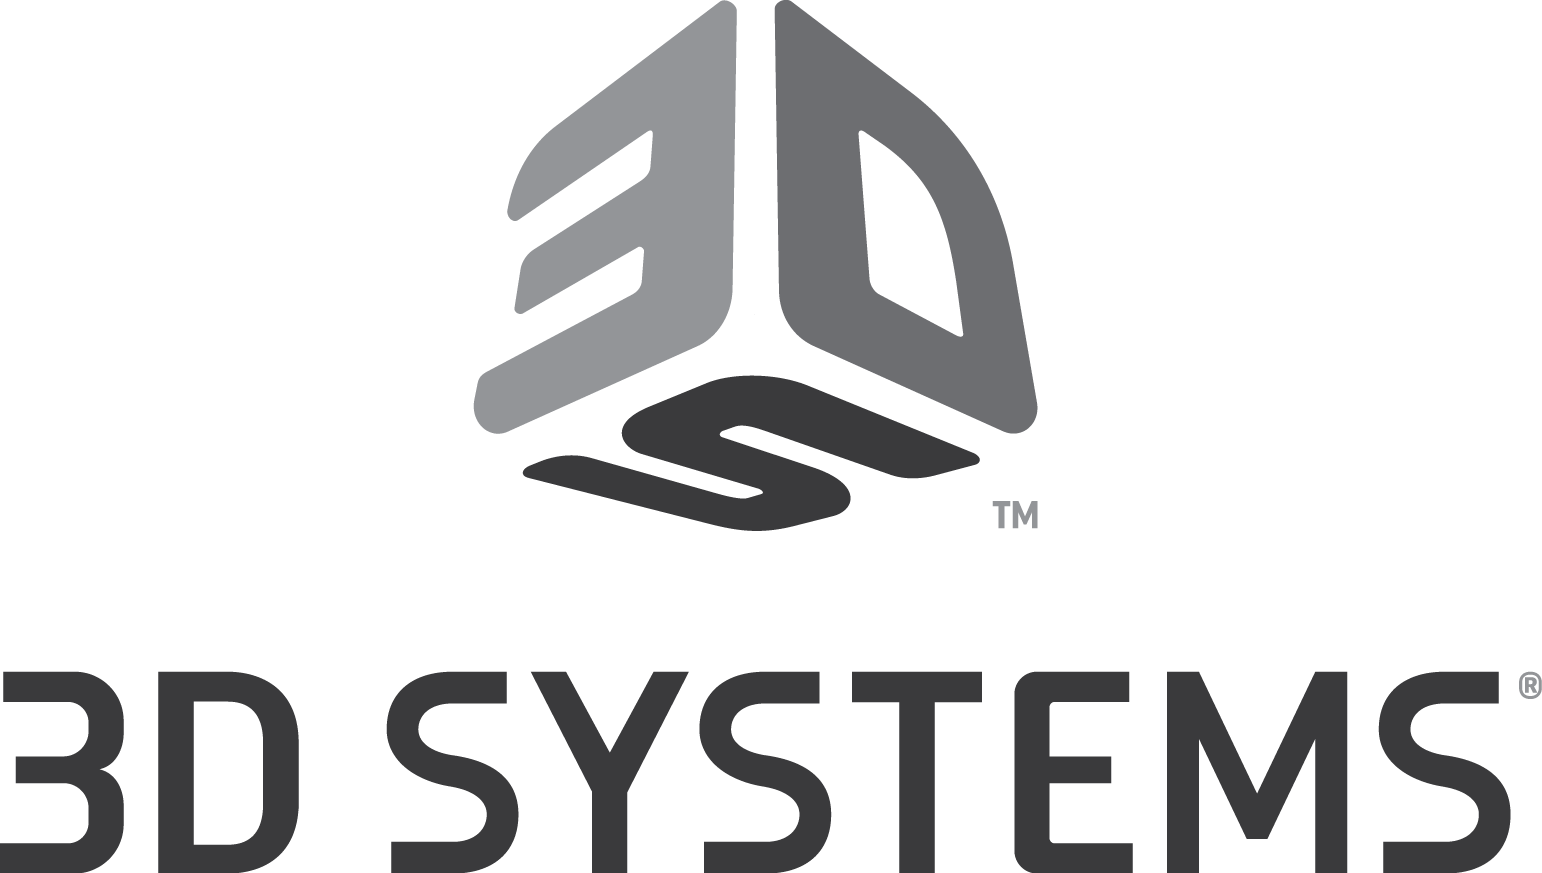
\includegraphics[width=0.9\textwidth]{figures/3D_Systems_Logo.png}
\caption{3D Systems Logo}
\end{figure}

\subsection{3D列印機:Creality K1 MAX}
本實驗選擇使用的3D列印機為Creality K1 MAX,以下為該機型的主要特點:
\begin{itemize}
	\item 大尺寸打印:使用CoreXY運動結構,高達300x300x300mm的列印面積,能夠滿足大型模型的列印需求。
	\item 解析度:具有極高的打印解析度,可以實現細膩的表面細節和精確的尺寸控制。
	\item 高速列印:配備了高效的運動系統和強大的驅動機構,最高能達到600mm/s的高速列印、20000mm/s²的加速度與32mm³/s 的超大流量,能夠顯著縮短列印時間。
	\item 耗材多樣性:支援多種列印耗材,包括PLA、ABS、TPU等,為使用者提供了更多創作自由度。
\end{itemize}

\begin{figure}[htbp]
    \centering
    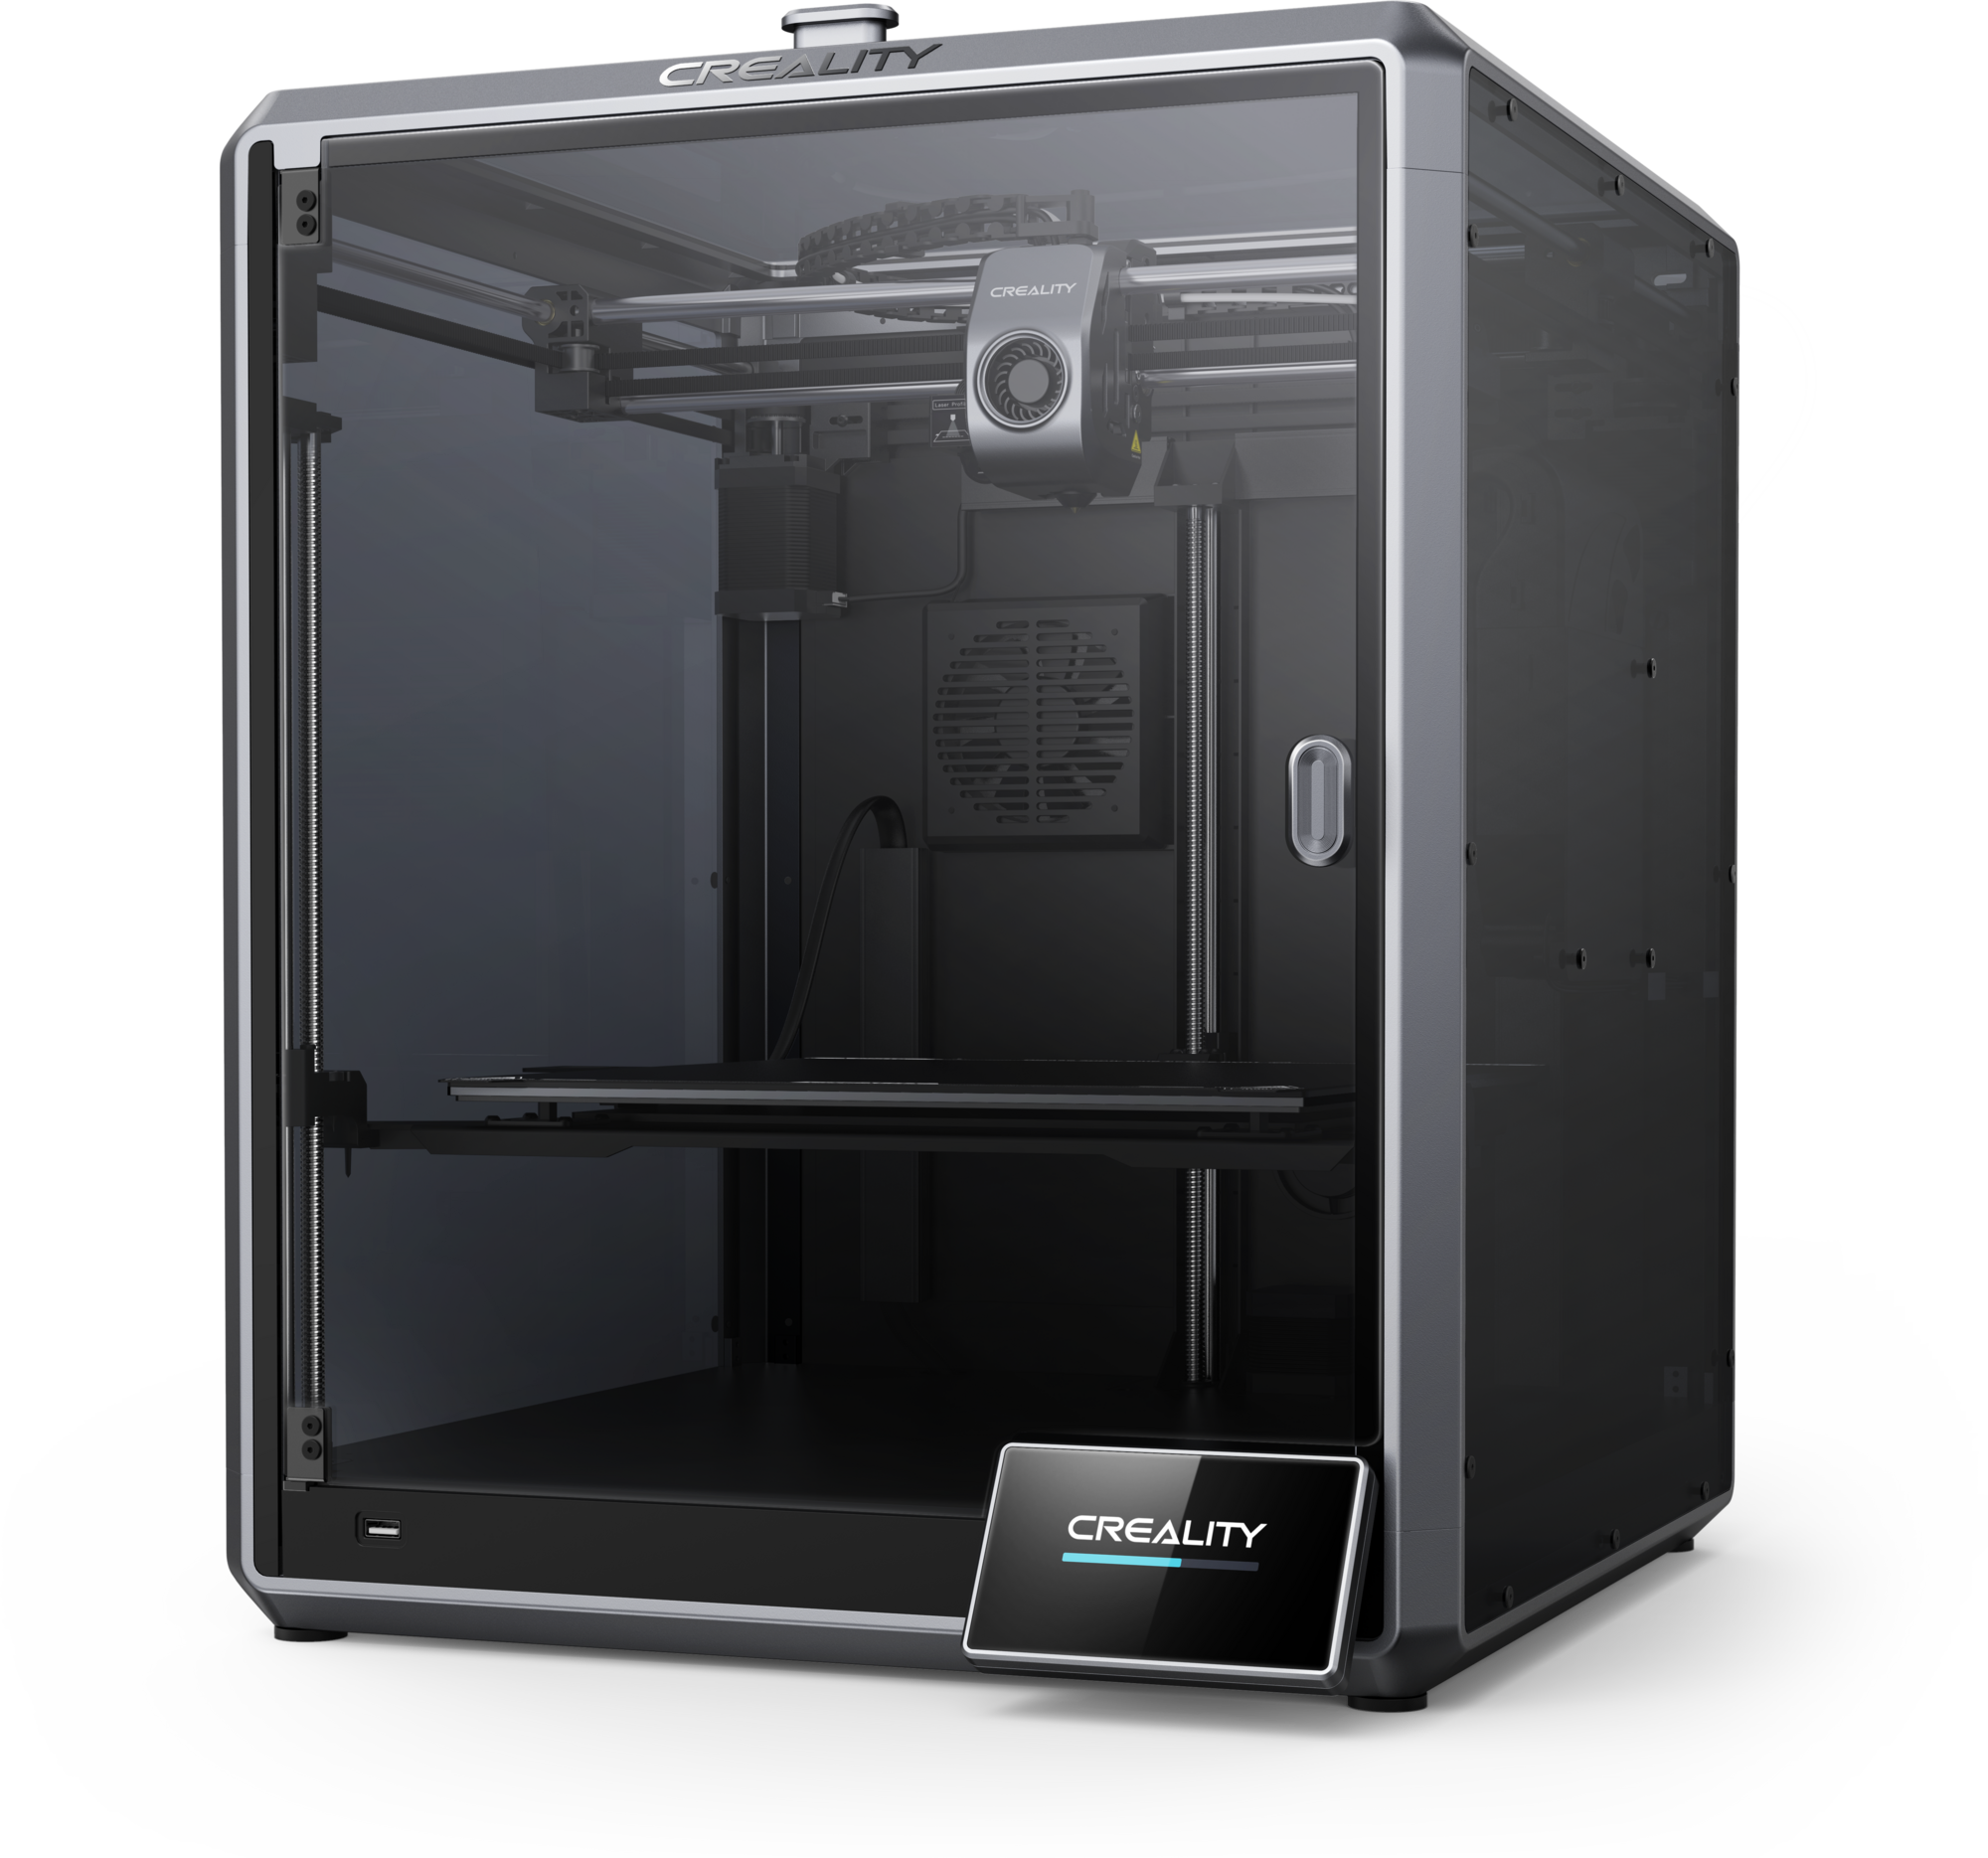
\includegraphics[width=0.9\textwidth]{figures/creality-k1-max.png}
\caption{Creality K1 MAX}
\end{figure}

\subsection{馬達與開發版介紹}
以下為本論文使用到的零件簡介:

1. SG90,是一款微型伺服馬達,由於扭矩較小,所以本實驗將其用於機械臂後段(頂點)。它的特點包括:
\begin{itemize}
	\item 重量:小巧輕便,重量僅為9克。
	\item 操作電壓:4.8V至6.0V。
	\item 扭矩:在4.8V時可達1.8kg/cm。
	\item 控制方式:使用PWM信號來控制轉角,通常範圍為0°至180°。
\end{itemize}

2. MG90S,是一款金屬齒輪伺服馬達,由於扭矩適中,所以本實驗將其用於機械臂前中段。其特點包括:
\begin{itemize}
	\item 重量:重量約為14g,稍大於SG90,但仍屬於微型伺服馬達。
	\item 操作電壓:4.8V至6.0V。
	\item 扭矩:在4.8V時可達2.2kg/cm。
	\item 控制方式:使用PWM信號來控制轉角,通常範圍為0°至180°。
\end{itemize}

3. MG996R,是一款高扭矩伺服馬達,由於扭矩較大,所以本實驗將其用於機械臂前段。其主要特點包括:
\begin{itemize}
	\item 尺寸:重量約為55g,適用於中型或大型專案。
	\item 操作電壓:4.8V至7.2V。
	\item 扭矩:在6.0V時可達9.4kg/cm。
	\item 控制方式:使用PWM信號來控制轉角,通常範圍為0°至180°。
\end{itemize}

4. Raspberry Pi 4,是一款高性能的嵌入式裝置。其主要特點包括:
\begin{itemize}
	\item 處理器:四核ARM Cortex-A72,1.5GHz。
	\item 內存:有2GB、4GB和8GB可選,本實驗採用8GB內存。
	\item 輸入/輸出:支援USB 3.0、HDMI、GPIO、以太網等連接方式,同時也支援wifi藍芽等無線連接方式
	\item 作業系統:本實驗採用Raspberry Pi OS(基於Debian)。
\end{itemize}

5. ESP32-S3-Devkit,是一款高性能、低功耗的微控制器,適合用於物聯網應用。其主要特點包括:
\begin{itemize}
	\item 處理器:雙核Xtensa LX7,最高240MHz。
	\item 內存:512KB SRAM,支持外部RAM擴展。
	\item 輸入/輸出:支援microUSB連接方式,同時也支援Wi-Fi和藍芽等無線連接方式。
	\item 作業系統:本實驗採用circuit python。
\end{itemize}

6. ESP32 Doit-Devkit,是一個常見的ESP32開發板,設計簡單且功能強大。其主要特點包括:
\begin{itemize}
	\item 處理器:雙核Xtensa LX6,最高240MHz。
	\item 內存:520KB SRAM。
	\item 支援microUSB連接方式,同時也支援Wi-Fi和藍芽等無線連接方式。
	\item 作業系統:本實驗採用circuit python。
\end{itemize}

7. L298N,直流馬達驅動模組,常用於控制雙馬達系統,本實驗將此裝置用於控制車輪。其主要特點包括:
\begin{itemize}
	\item 電壓範圍:可操作電壓範圍為5V至35V。
	\item 電流:每通道峰值電流可達2A。
	\item 控制:使用PWM訊號控制馬達速度和方向。
\end{itemize}

8. PCA9685,是一款16通道PWM驅動模組,通常用於控制伺服馬達和LED燈,本實驗將此裝置用於控制機械臂馬達。其主要特點包括:
\begin{itemize}
	\item PWM頻率:可調頻率範圍為24Hz至1526Hz。
	\item 接口:使用I2C介面進行訊號傳輸。
	\item 控制:使用PWM訊號控制馬達速度和方向,適合需要一次性控制大量馬達的專案。
\end{itemize}

\begin{figure}[!hbt]
    \centering
    \subcaptionbox
        {SG90
        \label{fig:fig-dataset-contrast-after-adjustment}}
        {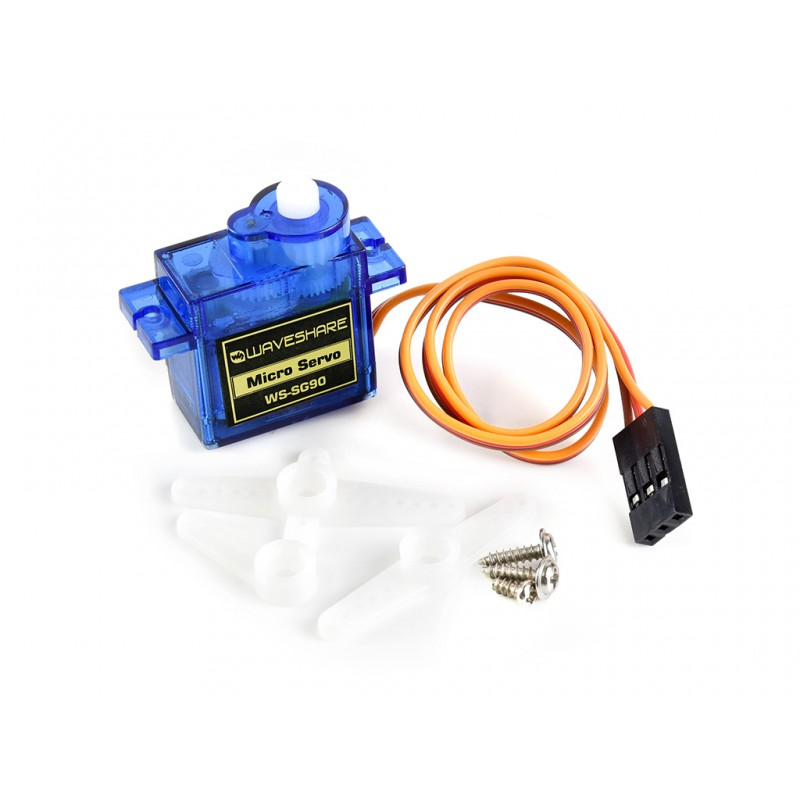
\includegraphics[width=0.25\linewidth]{figures/SG90.jpg}}
    ~    
    \subcaptionbox
        {MG90S
        \label{fig:fig-dataset-contrast-after-adjustment}}
        {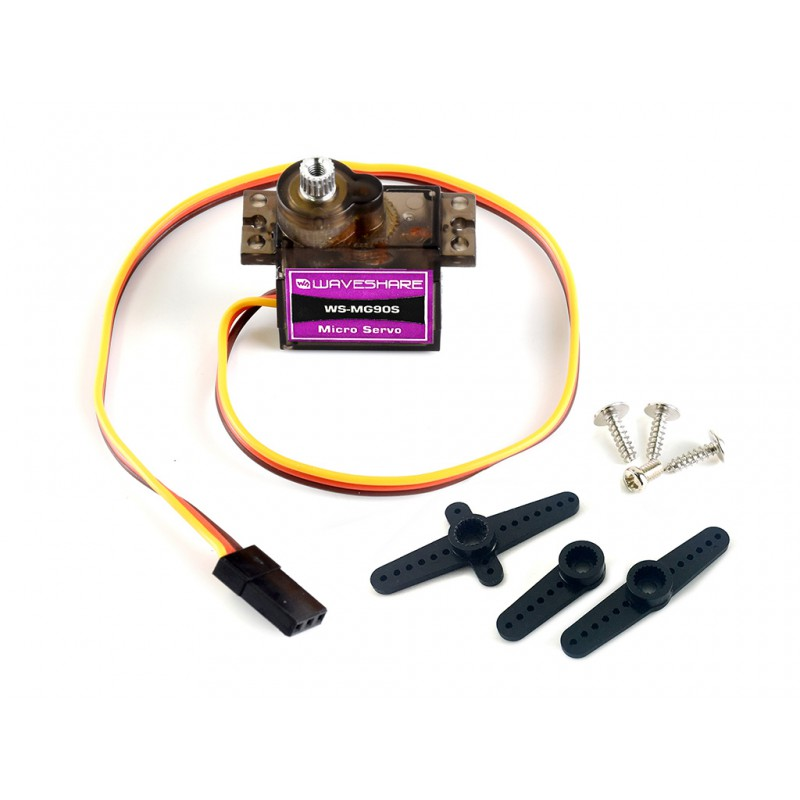
\includegraphics[width=0.25\linewidth]{figures/MG90S.jpg}}
    ~    
    \subcaptionbox
        {MG996R
        \label{fig:fig-dataset-contrast-after-adjustment}}
        {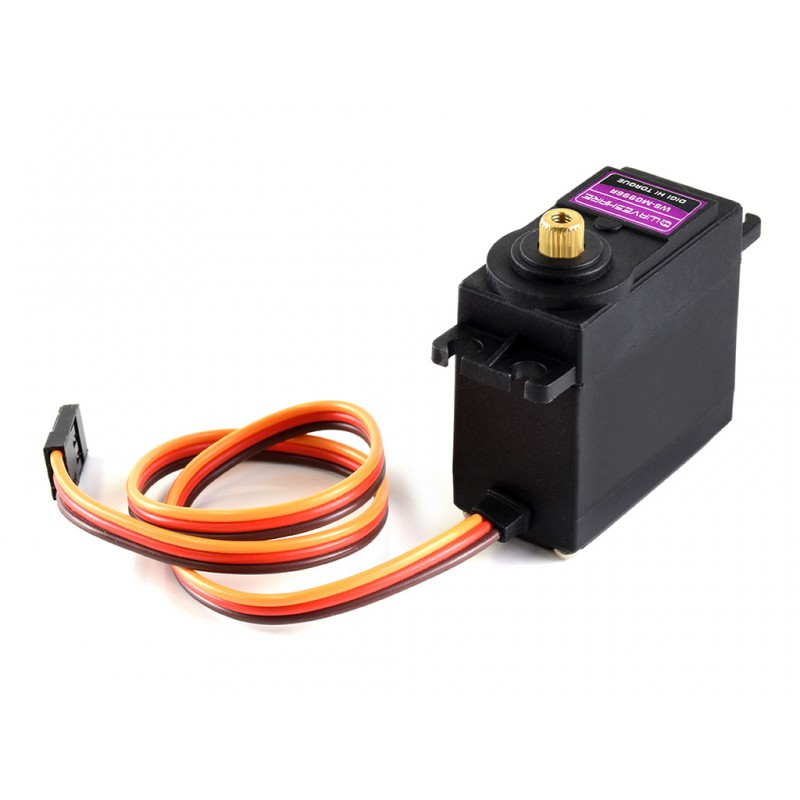
\includegraphics[width=0.25\linewidth]{figures/MG996R.jpg}}
    ~   
    \subcaptionbox
        {Raspberry Pi 4
        \label{fig:fig-dataset-contrast-after-adjustment}}
        {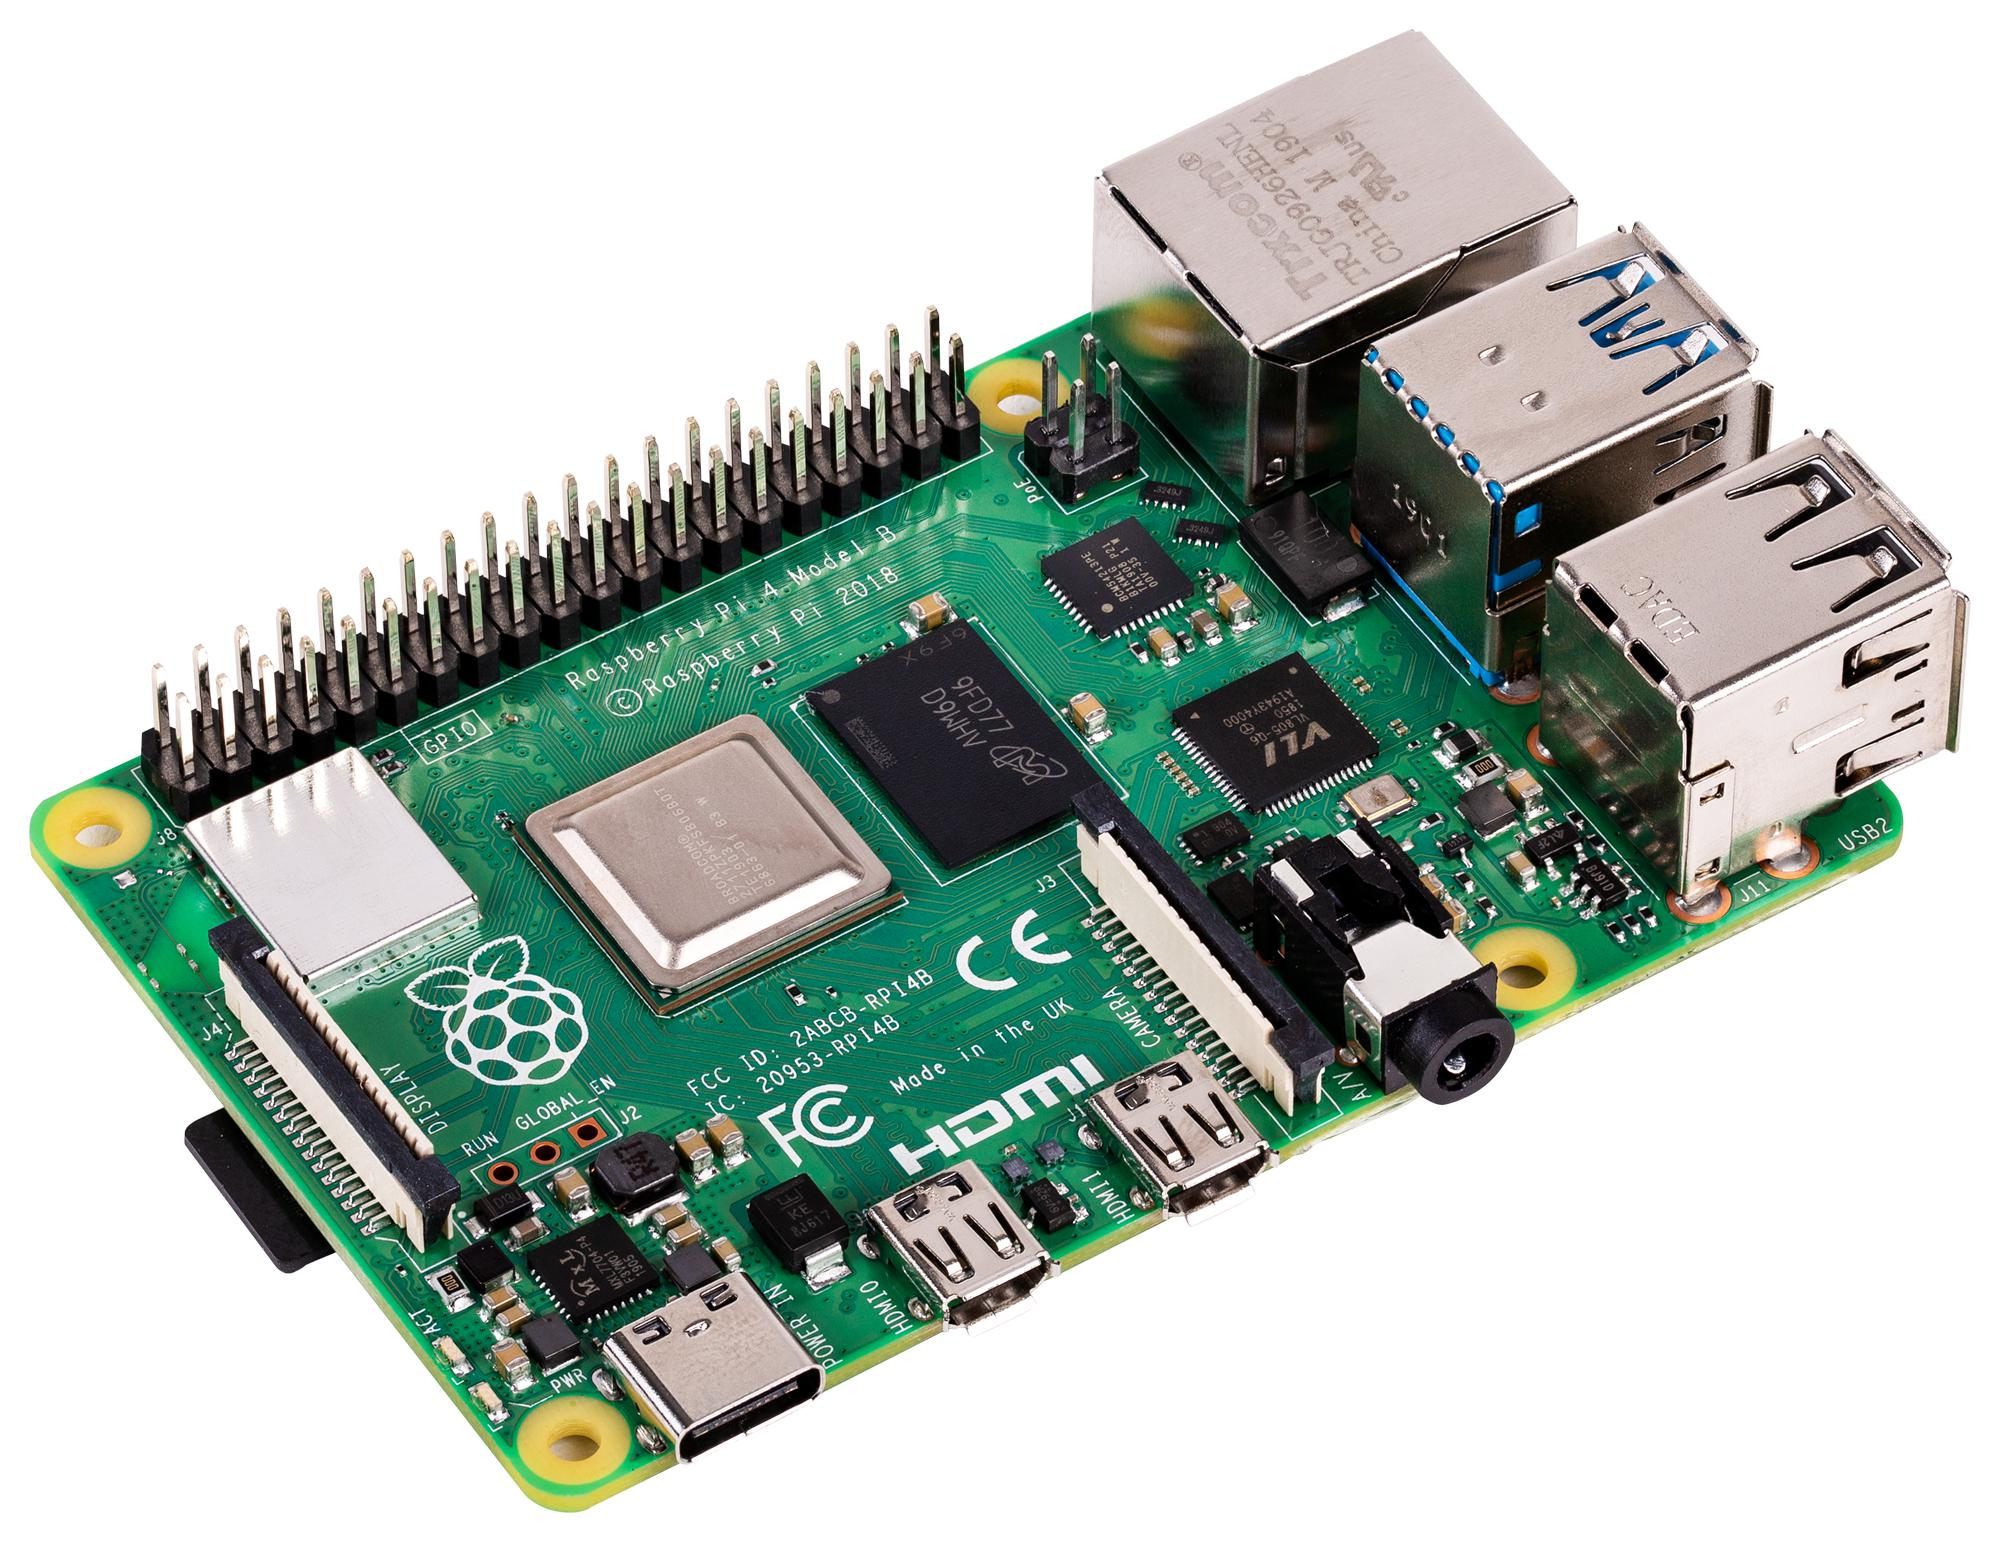
\includegraphics[width=0.25\linewidth]{figures/Rasberry pi 4.jpg}}
    ~    
    \subcaptionbox
        {ESP32-S3-Devkit
        \label{fig:fig-dataset-contrast-after-adjustment}}
        {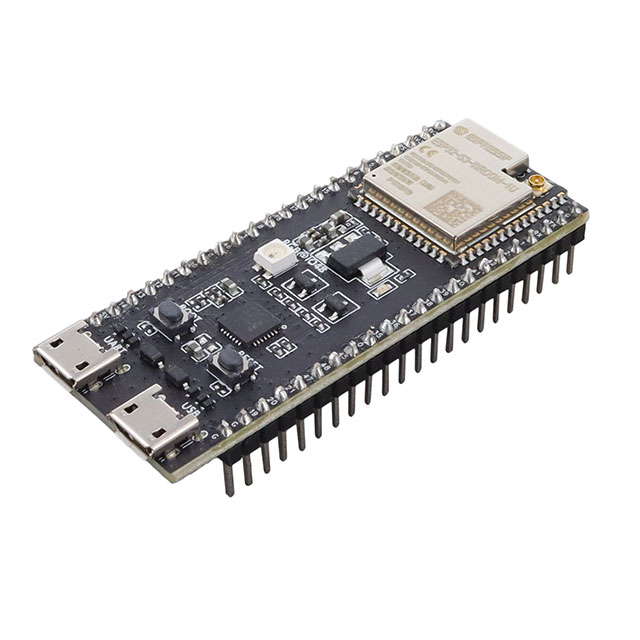
\includegraphics[width=0.25\linewidth]{figures/ESP32-S3.jpg}}
    ~    
    \subcaptionbox
        {ESP32 Doit-Devkit
        \label{fig:fig-dataset-contrast-after-adjustment}}
        {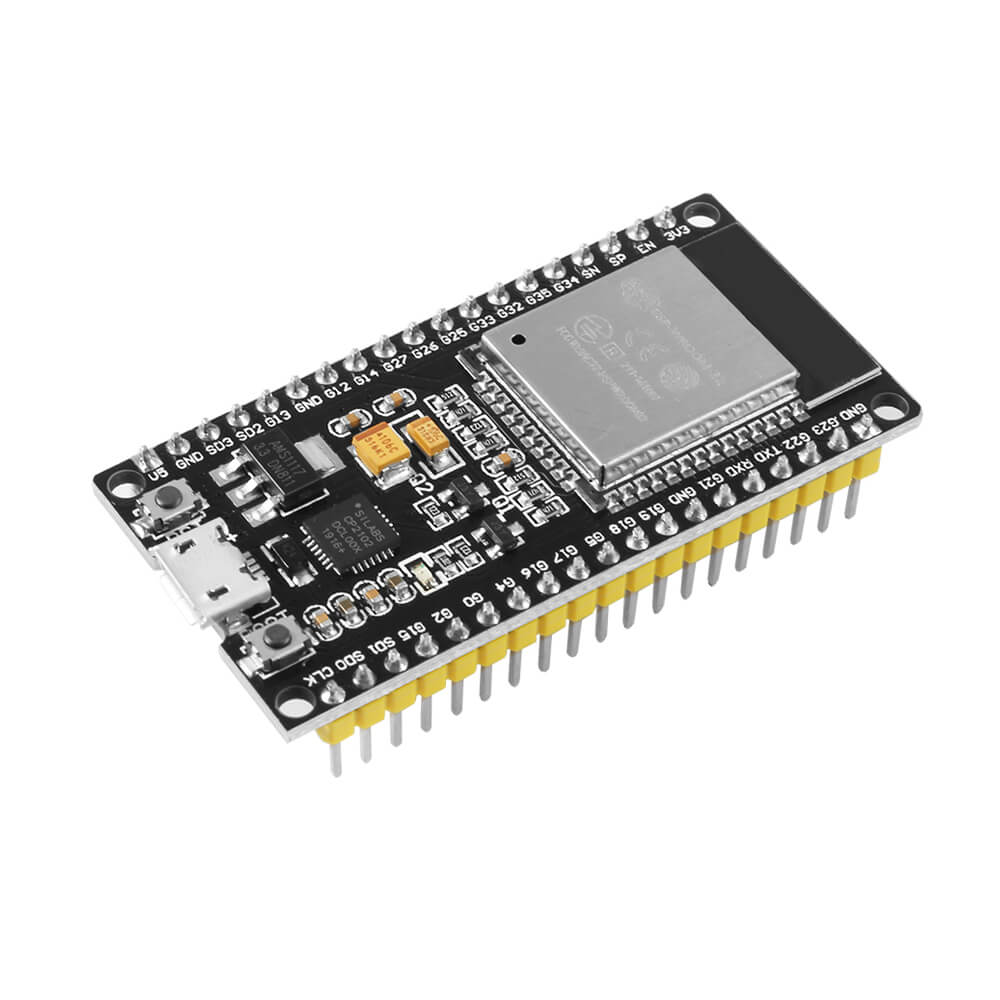
\includegraphics[width=0.25\linewidth]{figures/ESP32-DOIT.jpg}}
    ~  
    \subcaptionbox
        {L298N
        \label{fig:fig-dataset-contrast-after-adjustment}}
        {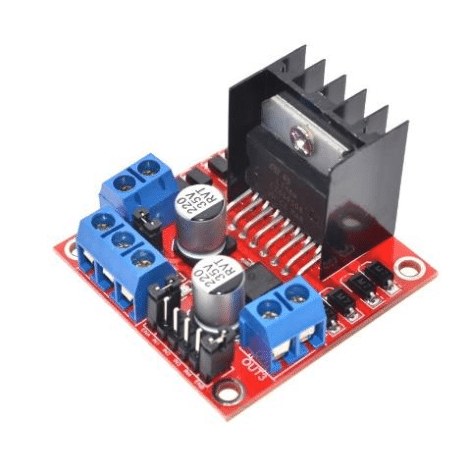
\includegraphics[width=0.25\linewidth]{figures/L298N.png}}
    ~    
    \subcaptionbox
        {PCA9685
        \label{fig:fig-dataset-contrast-after-adjustment}}
        {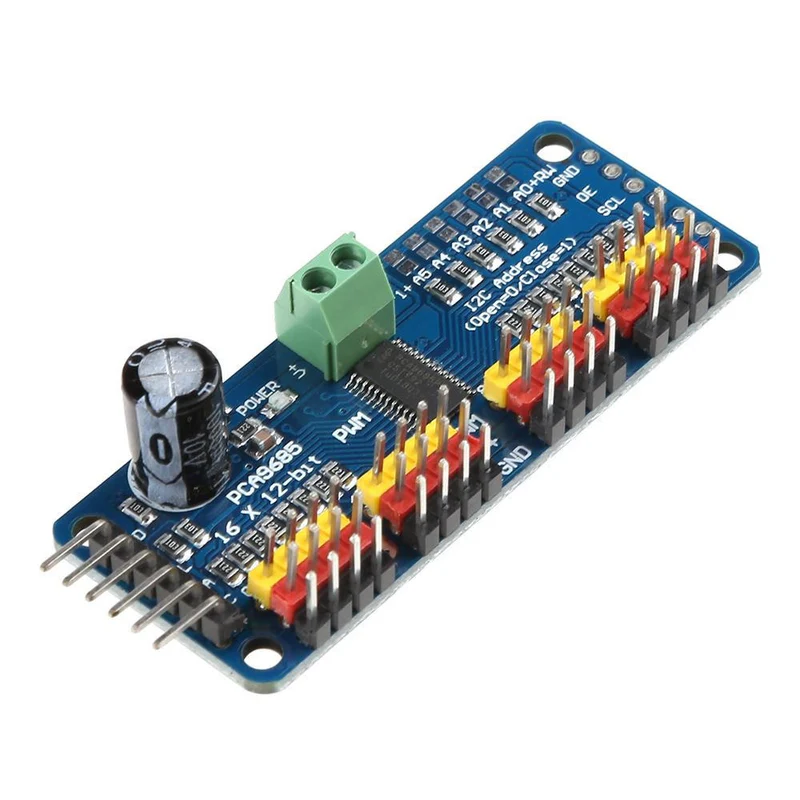
\includegraphics[width=0.25\linewidth]{figures/PCA9685.png}}
\caption{實驗一:實驗過程縮圖}
\end{figure}

\section{運動學開發}

\subsection{運動模擬環境}
本專案使用Python語言開發了一個簡易的機械臂模擬環境。這個模擬環境的基本原理,是將機械臂定義為一個擁有多個可調整參數的獨立物件,其中包括力臂長度、扭轉角、節點偏移、節點角度、目標頂點、和目前頂點等。這些參數可以由使用者根據需求進行調整,從而在虛擬空間中生成機械臂的模型。該模擬環境提供了一個直觀且靈活的介面,使得使用者能夠方便地設計和測試機械臂的運動行為。

\begin{listing}
    \begin{minted}[frame=single,
                   framesep=3mm,
                   linenos=true,
                   xleftmargin=21pt,
                   tabsize=4]{python}

        class ArmEnv_3D:
            def __init__(self, lList, vision=True):
                self.Link_length = lList
                self.Link_offset=[0]*len(lList)
                self.Twist_angle=[0]*len(lList)
                self.Joint_angle = [0]*len(lList)
                self.Target_point=[0, 0, 0]
                self.Current_point=[0, 0, sum(lList)]

            def Forward_kinematics(self, joint_angles):...
            
            def Geometric_solution(self):...

            def Gradient_policy(self,times=100, points=10, speed=5):...

            def initPicture(self):...

            def updatePicture(self):...

    \end{minted}
\caption{運動模擬環境程式架構} 
\end{listing}

\subsection{順向運動學}
在順向運動學部分,本專案採用了Denavit-Hartenberg方法作為主要的計算方式。這種方法能夠系統地描述和計算機械臂的運動行為。模擬環境中的相關函式可以直接被呼叫,利用即時的機械臂參數來計算操作點的空間座標。計算結果會即時顯示在模擬空間中。

\subsection{逆向運動學}
在逆向運動學方面,本專案結合了幾何求解(Geometric solution approach)方法和策略梯度(Policy-Gradient solution approach)方法來進行計算。幾何求解方法主要用於計算運動模式較為簡單的機械臂,而策略梯度方法則適用於運動較為複雜的機械臂。這些計算函式同樣可以在模擬環境中直接被呼叫。根據輸入的目標操作點位置,系統會計算出對應的扭轉角,並將結果顯示在模擬空間中。

\section{大型語言模型選擇}
\subsection{open ai介紹}
\subsection{下prompt的規則}

\section{系統架構}
\subsection{系統架構圖}
整個系統架構介紹
\subsection{client端的輸入內容}
\subsection{轉換到code的過程}

\end{document}